% ============================================================
%  APPENDICES  –  N4 Recovery System Interim Report
%  Minimal, image-focused appendix
% ============================================================
\appendix

% ------------------------------------------------------------
\section{Appendix A: CAD Drawings with Title Blocks}
\label{app:cad}

The engineering drawings below were produced in SolidWorks and include the institution title block, part number, material specification, and revision level required for fabrication.

\begin{figure}[H]
\centering
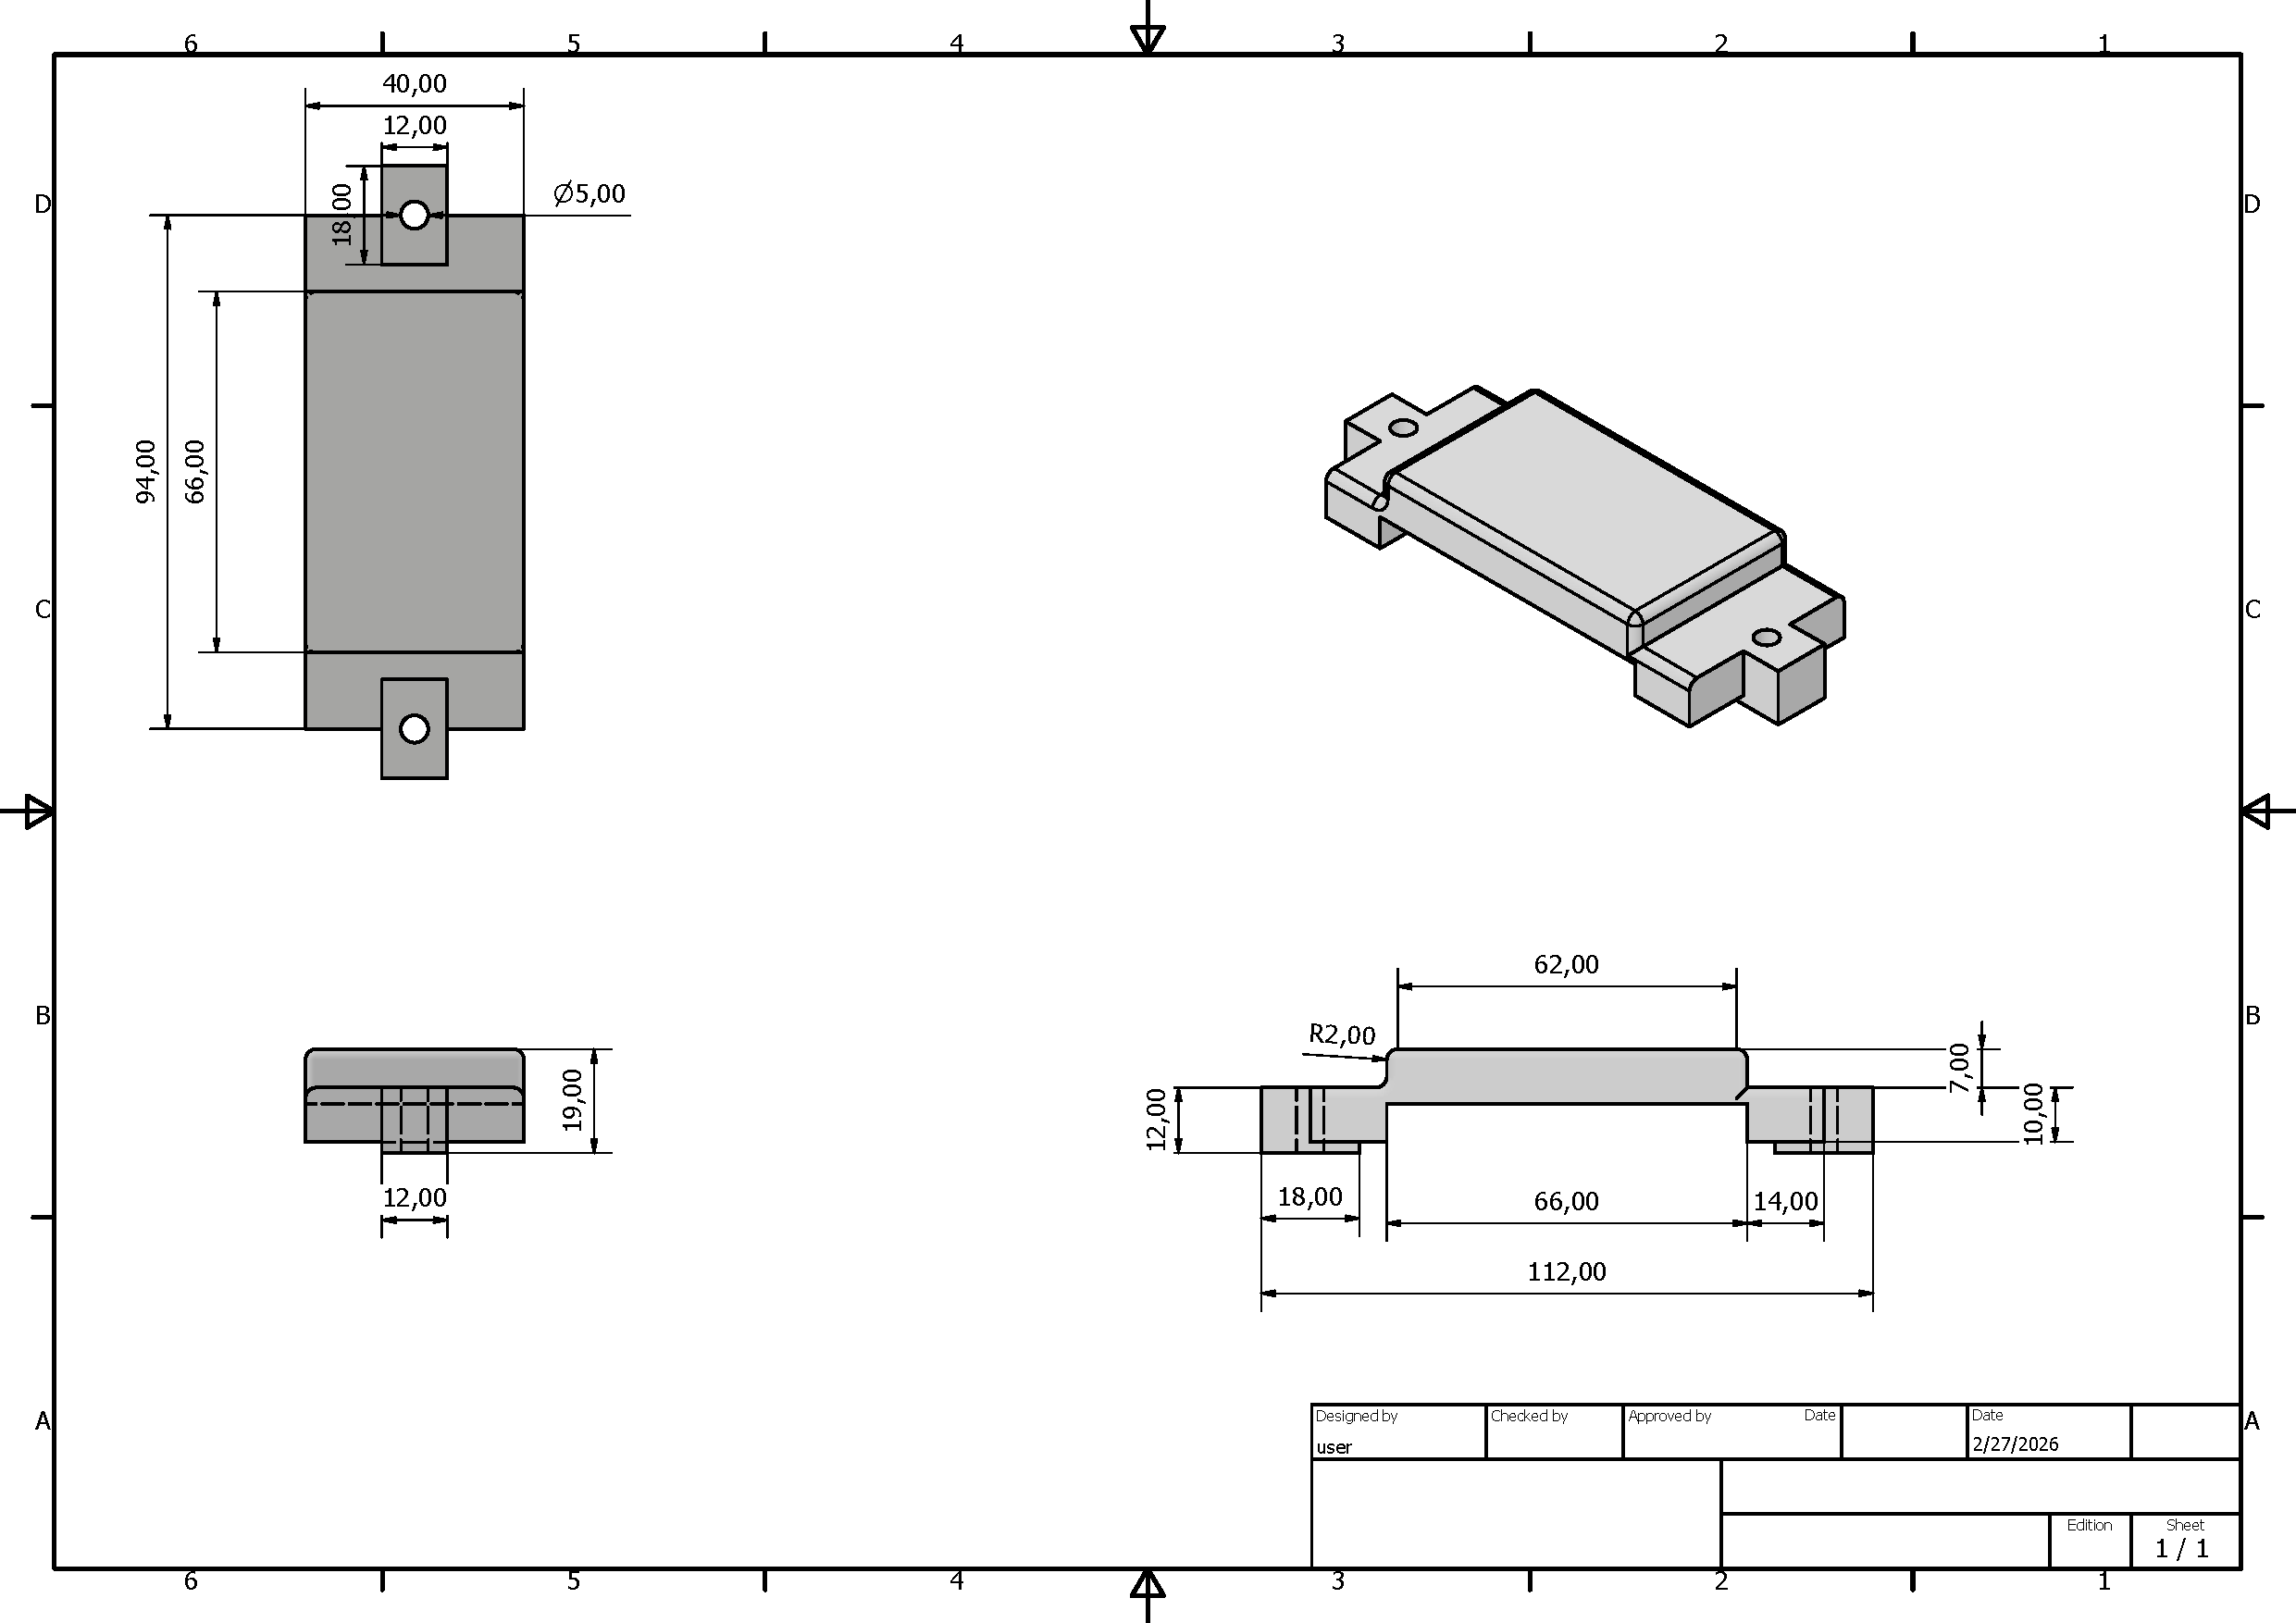
\includegraphics[width=\textwidth,page=1]{images/mechanical/18650_case_cover.pdf}
\caption{18650 battery case cover -- 2D manufacturing drawing with title block}
\label{fig:app_cad_case_cover}
\end{figure}

\begin{figure}[H]
\centering

\includegraphics[width=\textwidth,page=1]{images/mechanical/18650_case.pdf}
\caption{18650 battery case body -- 2D manufacturing drawing with title block}
\label{fig:app_cad_case_body}
\end{figure}

\begin{figure}[H]
\centering
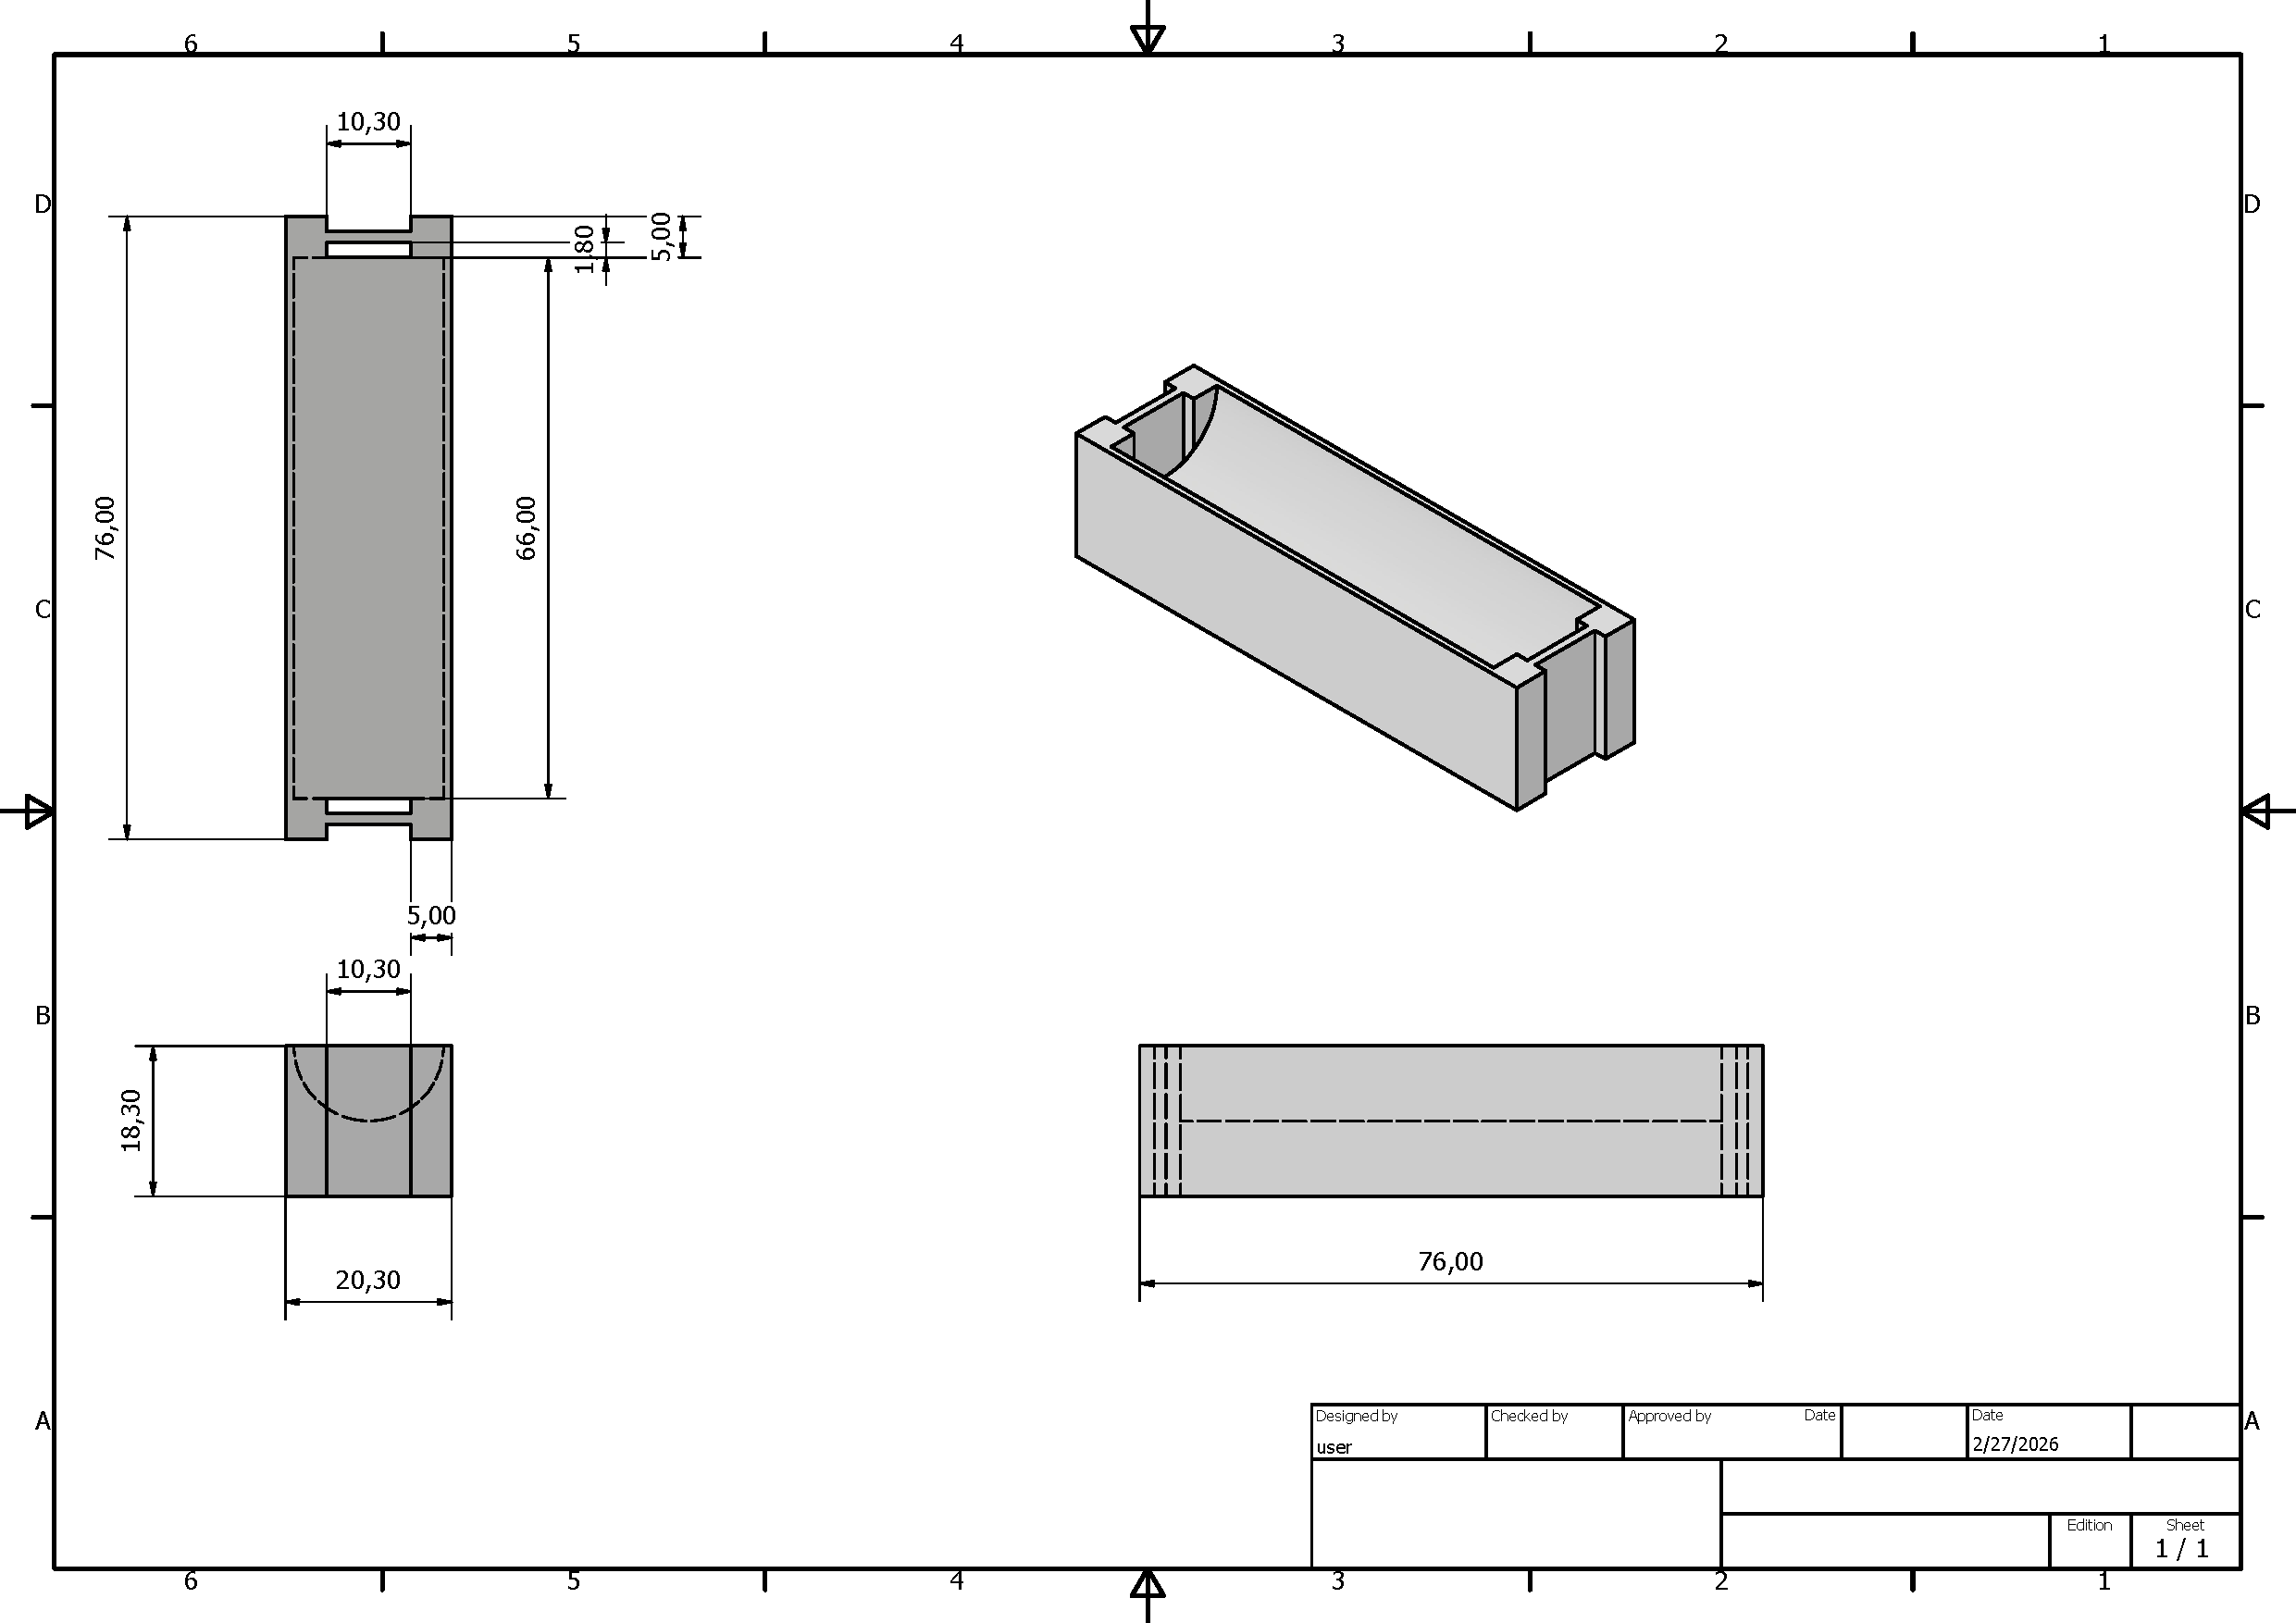
\includegraphics[width=\textwidth,page=1]{images/mechanical/Edge_Batt.pdf}
\caption{Edge battery support bracket -- 2D manufacturing drawing with title block}
\label{fig:app_cad_edge_batt}
\end{figure}

\begin{figure}[H]
\centering
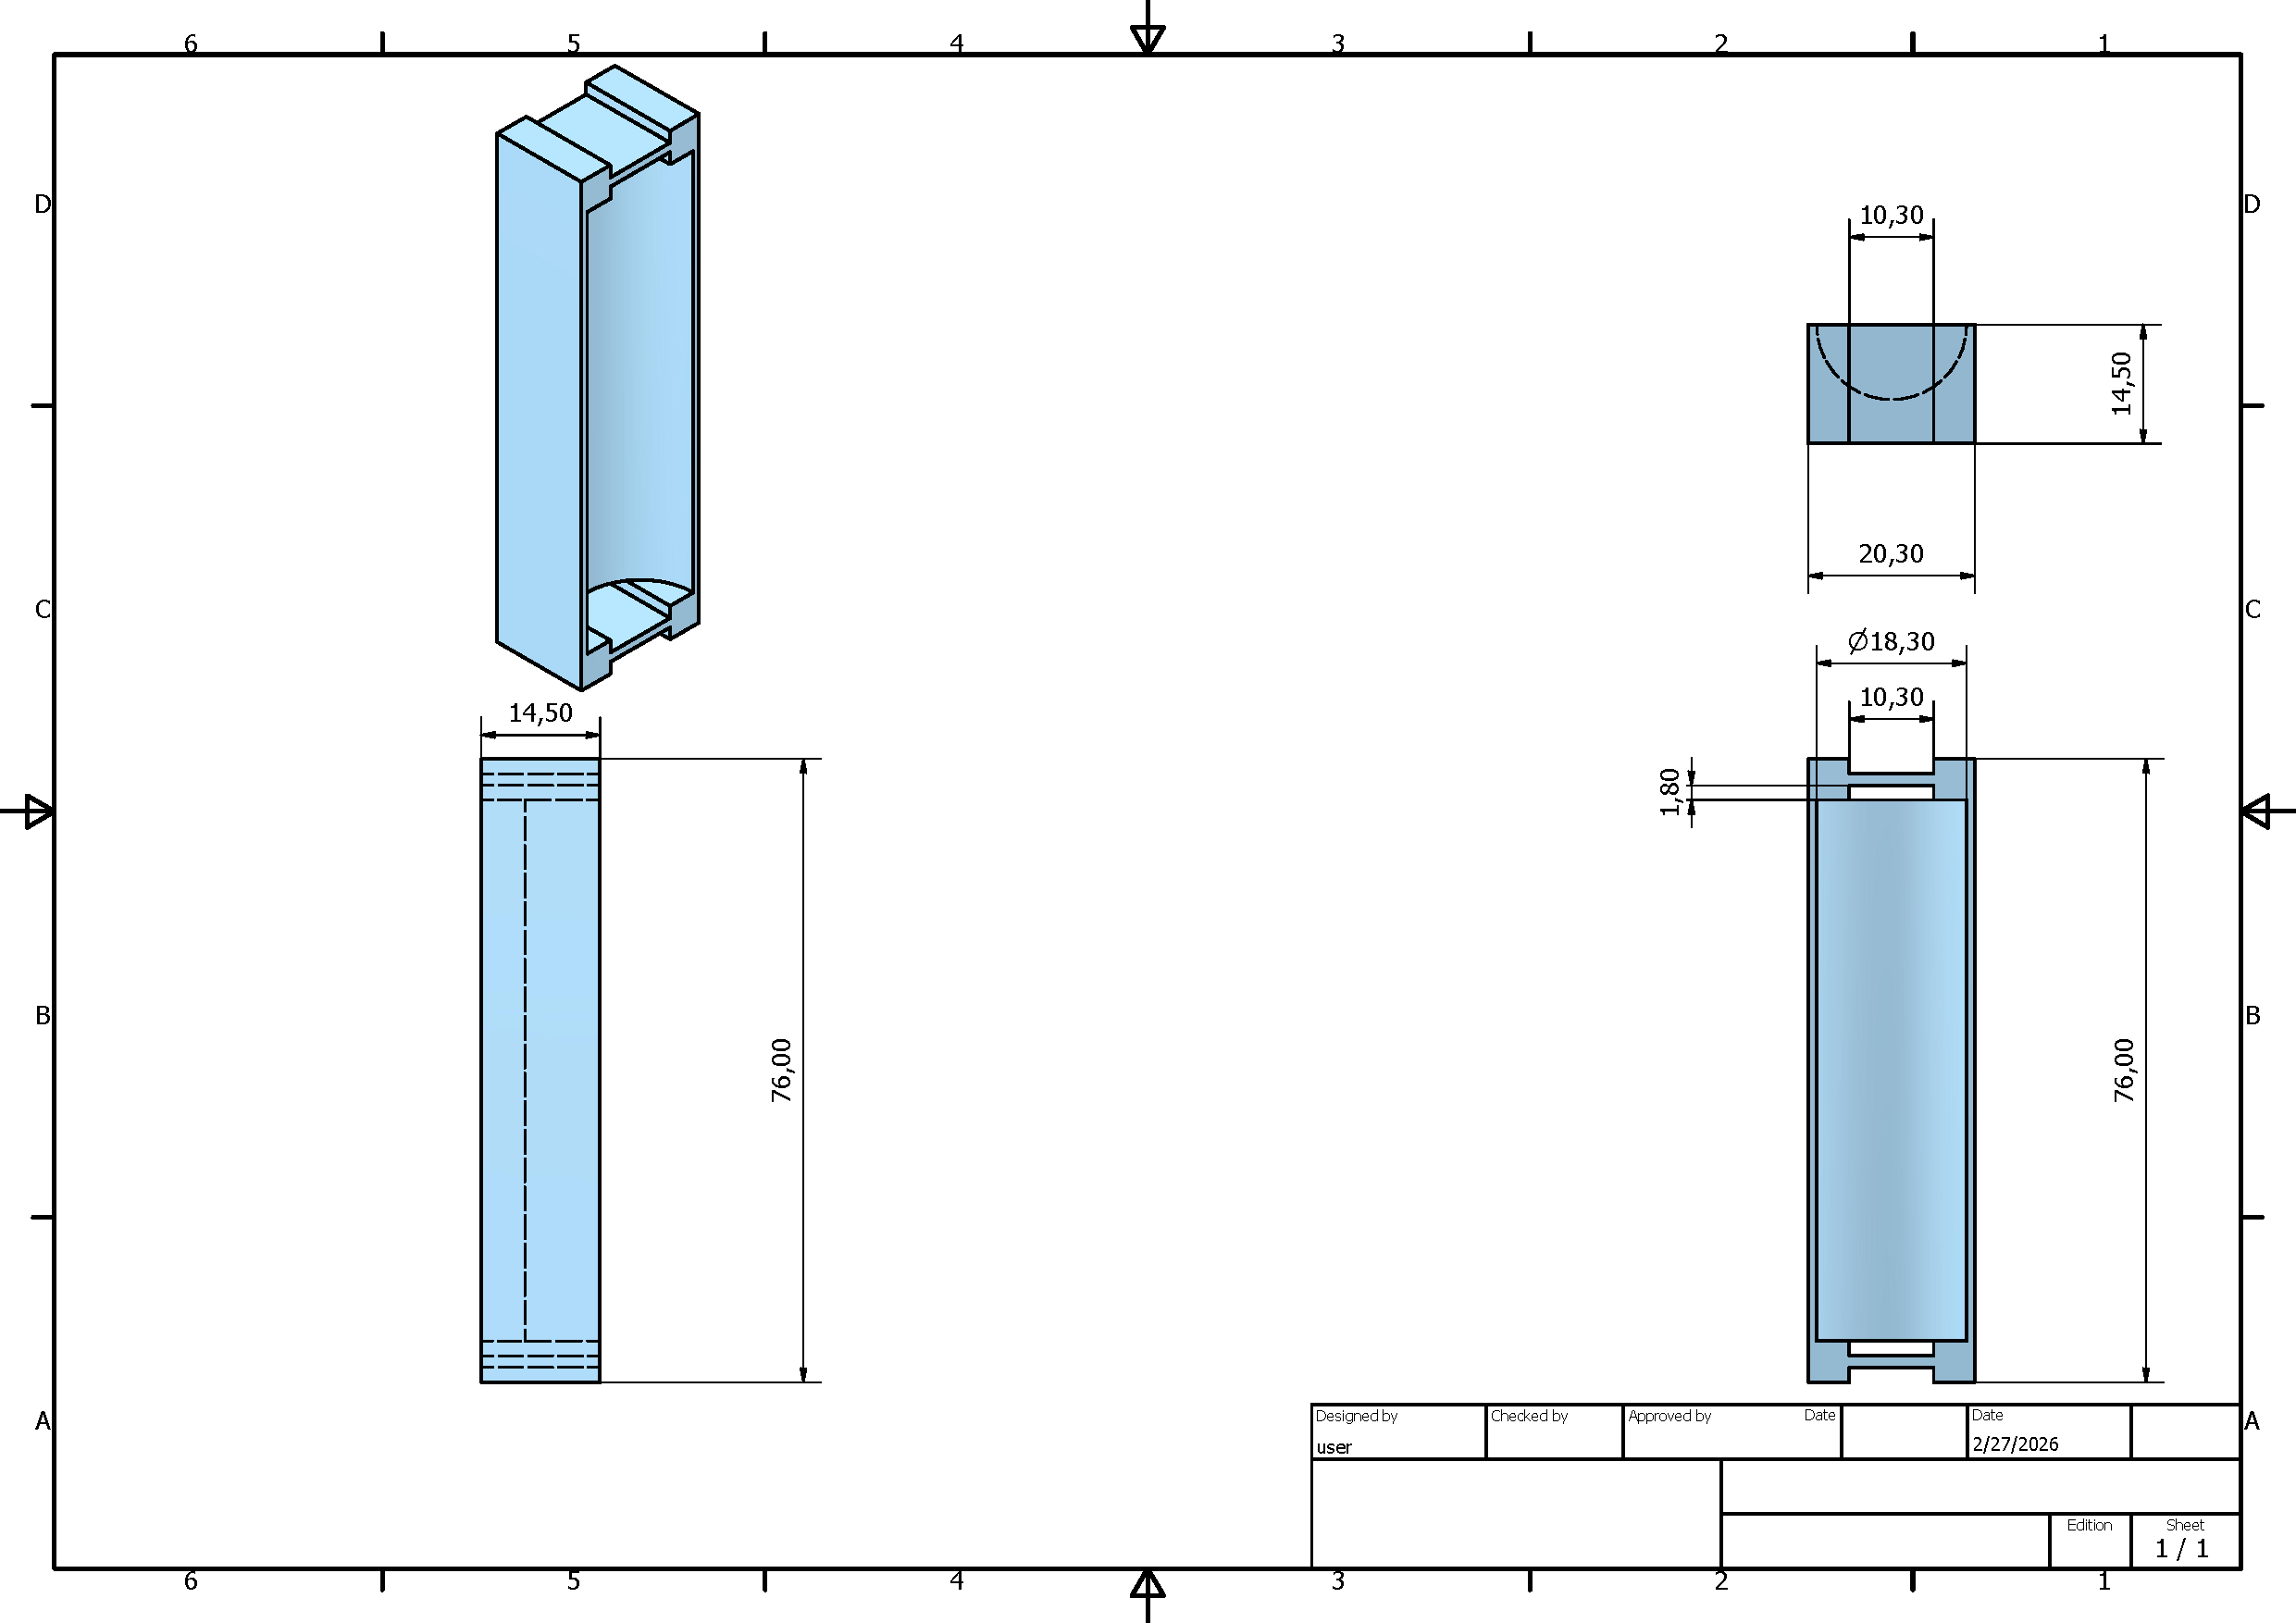
\includegraphics[width=\textwidth,page=1]{images/mechanical/mid_Batt.pdf}
\caption{Mid battery support bracket -- 2D manufacturing drawing with title block}
\label{fig:app_cad_mid_batt}
\end{figure}

% ------------------------------------------------------------
\section{Appendix B: Flight Computer Circuit Design Reference}
\label{app:fc_schematic}

Figure~\ref{fig:app_fc_easyeda} shows the current EasyEDA schematic for the flight computer, used as the design reference for PCB layout and component placement.

\begin{figure}[H]
\centering
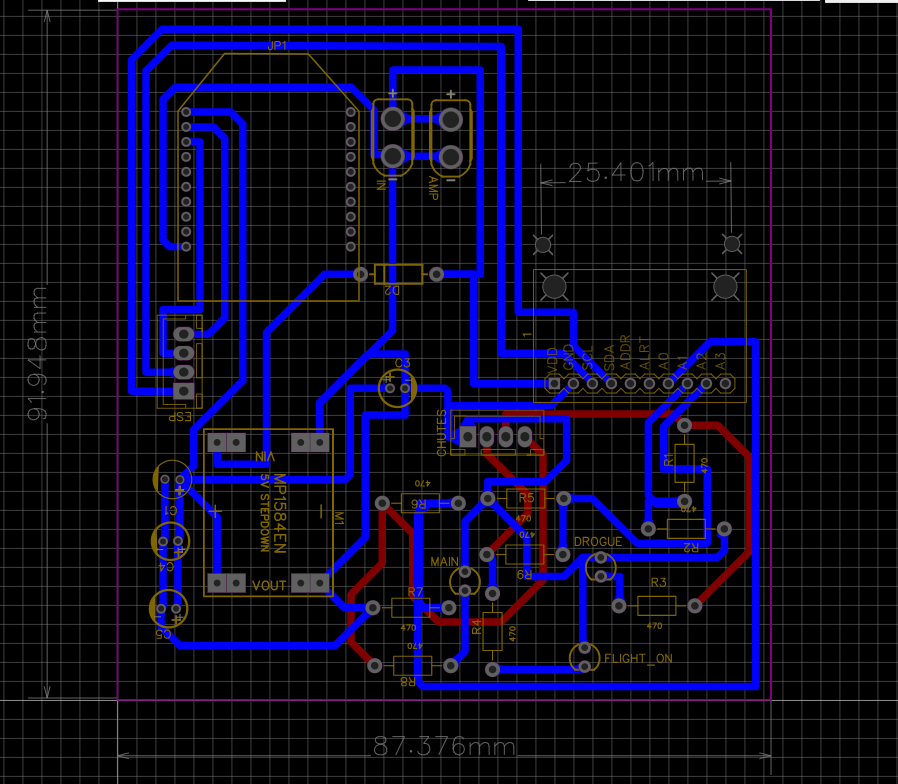
\includegraphics[width=\textwidth]{images/FC_Xbee_Design__easyDA.PNG}
\caption{Current flight computer EasyEDA schematic -- design reference for PCB fabrication (ESP32, XBee-PRO 900HP, power management, deployment circuitry)}
\label{fig:app_fc_easyeda}
\end{figure}

% ------------------------------------------------------------
\section{Appendix C: Project Budget}
\label{app:budget}

\begin{table}[H]
\centering
\caption{Project Budget Breakdown}
\small
\begin{tabular}{@{}p{4.5cm}|c|c|p{2cm}|c@{}}
\toprule
\rowcolor{gray!22}\textbf{Item} & \textbf{Qty} & \textbf{Unit Cost (KES)} & \textbf{Total (KES)} & \textbf{Status} \\ \midrule
ESP32-WROOM-32              & 2  & 1800   & 3600  & Received    \\
XBee-PRO 900HP              & 2  & 4,500 & 9,000  & Received    \\
4S Lithium ion batteries (30000 mAh) & 4  & 500 & 2000  & Received    \\
BMS Board (4S)              & 3  & 650   & 1,950  & Received    \\
IRLZ44N MOSFET              & 10 & 45    & 450    & Received    \\
Nichrome Wire (10 m)        & 1  & 500   & 500    & Received    \\
PCB Fabrication (5 pcs)     & 1  & 4,500 & 4,500  & Fabrication \\
PCB Components (R, C, etc.) & 1  & 2,000 & 2,000  & Partial     \\
PETG Filament (1 kg)        & 1  & 1,800 & 1,800  & Received    \\
Crimson Powder (100 g)        & 1  & 500   & 500    & Pending     \\
Connectors (XT60, JST, etc.)& 1  & 1,200 & 1,200  & Received    \\
Fasteners and Hardware      & 1  & 800   & 800    & Partial     \\
Miscellaneous               & 1  & 1,500 & 1,500  & --          \\ \midrule
\multicolumn{2}{r|}{\textbf{Total Estimated Cost:}} & & \textbf{37,300} & -- \\ \bottomrule
\end{tabular}
\end{table}

% ------------------------------------------------------------
\section{Appendix D: Project Timeplan}
\label{app:timeplan}

\begin{figure}[H]
\centering
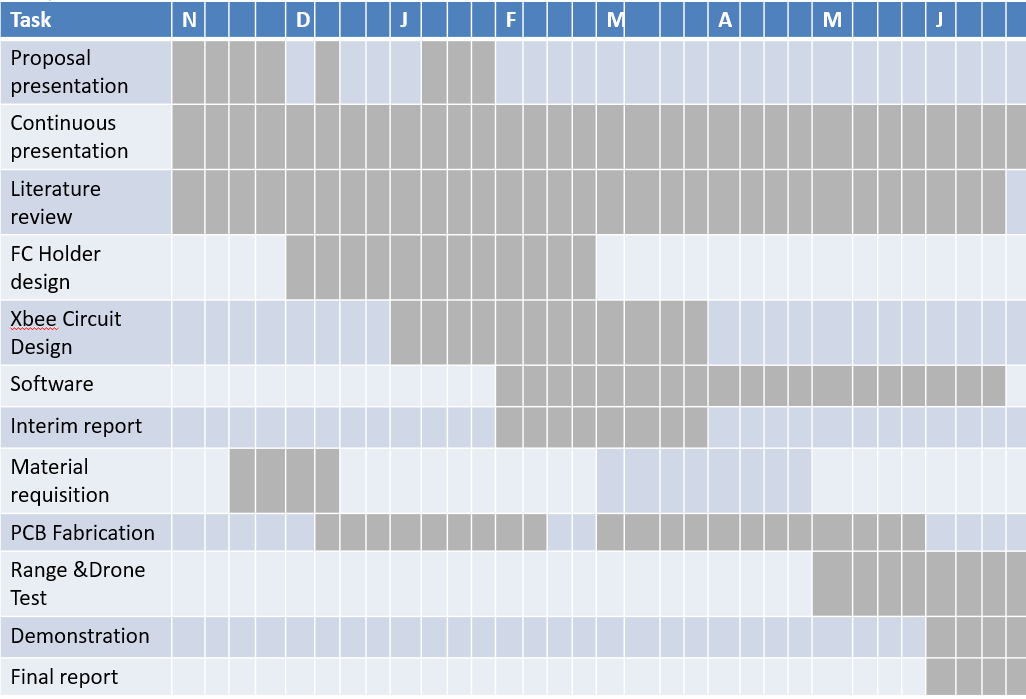
\includegraphics[width=\textwidth]{images/Timeplan.PNG}
\caption{N4 recovery system project Gantt chart showing planned phases, milestones, and current progress}
\label{fig:app_timeplan}
\end{figure}

% ============================================================
%  END OF APPENDICES
% ============================================================